%%%%%%%%%%%%%%%%%%%%%%%%%%%%%%%%%%%%%%%%%%%%%%%%%%%%%%%%%%%%%%%%%%%%%%%%%%%%%%%%
%  Document class
%%%%%%%%%%%%%%%%%%%%%%%%%%%%%%%%%%%%%%%%%%%%%%%%%%%%%%%%%%%%%%%%%%%%%%%%%%%%%%%%
\documentclass[final]{siamltex}

%%%%%%%%%%%%%%%%%%%%%%%%%%%%%%%%%%%%%%%%%%%%%%%%%%%%%%%%%%%%%%%%%%%%%%%%%%%%%%%%
%  Packages and styles
%%%%%%%%%%%%%%%%%%%%%%%%%%%%%%%%%%%%%%%%%%%%%%%%%%%%%%%%%%%%%%%%%%%%%%%%%%%%%%%%
\usepackage{graphicx}
\usepackage{cite}
\usepackage{color} 
\usepackage{algorithmic}
\usepackage{algorithm}
\usepackage{epsfig}
\usepackage{xspace}
\usepackage{amsfonts}
\usepackage{amsmath}
\usepackage{amssymb}
\usepackage{url}
\usepackage{listings}
\bibliographystyle{siam}

%%%%%%%%%%%%%%%%%%%%%%%%%%%%%%%%%%%%%%%%%%%%%%%%%%%%%%%%%%%%%%%%%%%%%%%%%%%%%%%%
%  PLoS stuff
%%%%%%%%%%%%%%%%%%%%%%%%%%%%%%%%%%%%%%%%%%%%%%%%%%%%%%%%%%%%%%%%%%%%%%%%%%%%%%%%
\topmargin 0.0cm
\oddsidemargin 0.5cm
\evensidemargin 0.5cm
\textwidth 16cm 
\textheight 21cm
\usepackage[labelfont=bf,labelsep=period,justification=raggedright]{caption}
\makeatletter
\renewcommand{\@biblabel}[1]{\quad#1.}
\makeatother
\date{}
\pagestyle{myheadings}


%%%%%%%%%%%%%%%%%%%%%%%%%%%%%%%%%%%%%%%%%%%%%%%%%%%%%%%%%%%%%%%%%%%%%%%%%%%%%%%%
%  Some useful commands
%%%%%%%%%%%%%%%%%%%%%%%%%%%%%%%%%%%%%%%%%%%%%%%%%%%%%%%%%%%%%%%%%%%%%%%%%%%%%%%%
\newcommand{\oh}[1]
    {\mbox{$ {\mathcal O}( #1 ) $}}
\newcommand{\eqn}[1]
    {(\ref{eqn:#1})}
\newcommand{\fig}[1]
    {Figure~\ref{fig:#1}}
\newcommand{\tabl}[1]
    {Table~\ref{tab:#1}}
\newcommand{\tab}[1]
    {Table~\ref{tab:#1}}
\newcommand{\figs}[1]
    {Figures~\ref{fig:#1}}
\newcommand{\cuda}
    {{\sc cuda}\xspace}
\newcommand{\namd}
    {{\sc namd}\xspace}
\newcommand{\acemd}
    {{\sc acemd}\xspace}
\newcommand{\fenzi}
    {{\sc fenzi}\xspace}
\newcommand{\mdcore}
    {{\tt mdcore}\xspace}
\newcommand{\swift}
    {{\sc swift}\xspace}
\newcommand{\bsf}[1]
    {\textbf{\textsf{#1}}}


%%%%%%%%%%%%%%%%%%%%%%%%%%%%%%%%%%%%%%%%%%%%%%%%%%%%%%%%%%%%%%%%%%%%%%%%%%%%%%%%
%  Title, author and affiliations
%%%%%%%%%%%%%%%%%%%%%%%%%%%%%%%%%%%%%%%%%%%%%%%%%%%%%%%%%%%%%%%%%%%%%%%%%%%%%%%%
\title{Efficient and Scalable Algorithms for Smoothed Particle Hydrodynamics on Multi-Core
    Architectures}
\author{Pedro Gonnet\thanks{School of Engineering and Computing Sciences,
    Durham University, Durham, Untied Kingdom ({\tt pedro.gonnet@durham.ac.uk}).}}

\begin{document}

%%%%%%%%%%%%%%%%%%%%%%%%%%%%%%%%%%%%%%%%%%%%%%%%%%%%%%%%%%%%%%%%%%%%%%%%%%%%%%%%
%  Set options for the listings package
%%%%%%%%%%%%%%%%%%%%%%%%%%%%%%%%%%%%%%%%%%%%%%%%%%%%%%%%%%%%%%%%%%%%%%%%%%%%%%%%
\lstset{%
    language=C,
    basicstyle=\small\tt,
    numbers=left,
    numberstyle=\tiny
    }


%%%%%%%%%%%%%%%%%%%%%%%%%%%%%%%%%%%%%%%%%%%%%%%%%%%%%%%%%%%%%%%%%%%%%%%%%%%%%%%%
%  Title and Author
%%%%%%%%%%%%%%%%%%%%%%%%%%%%%%%%%%%%%%%%%%%%%%%%%%%%%%%%%%%%%%%%%%%%%%%%%%%%%%%%
% Title must be 150 characters or less
\maketitle


%%%%%%%%%%%%%%%%%%%%%%%%%%%%%%%%%%%%%%%%%%%%%%%%%%%%%%%%%%%%%%%%%%%%%%%%%%%%%%%%
%  Abstract
%%%%%%%%%%%%%%%%%%%%%%%%%%%%%%%%%%%%%%%%%%%%%%%%%%%%%%%%%%%%%%%%%%%%%%%%%%%%%%%%
\begin{abstract}
A new framework for the parallelization of Smoothed Particle Hydrodynamics (SPH)
simulations on shared-memory parallel architectures is described.
This framework relies on fast and cache-efficient cell-based neighbour-finding
algorithms, as well as task-based parallelism to achieve good scaling and
parallel efficiency on multi-core computers.
\end{abstract}


%%%%%%%%%%%%%%%%%%%%%%%%%%%%%%%%%%%%%%%%%%%%%%%%%%%%%%%%%%%%%%%%%%%%%%%%%%%%%%%%
%  Metadata
%%%%%%%%%%%%%%%%%%%%%%%%%%%%%%%%%%%%%%%%%%%%%%%%%%%%%%%%%%%%%%%%%%%%%%%%%%%%%%%%
\begin{keywords} 
smoothed particle hydrodynamics,
simulation,
task-based parallelism,
multi-cores
\end{keywords}

\begin{AMS}
15A15, 15A09, 15A23
\end{AMS}

\pagestyle{myheadings}
\thispagestyle{plain}
\markboth{P. GONNET}{EFFICIENT AND SCALABLE ALGORITHMS FOR SPH}


%%%%%%%%%%%%%%%%%%%%%%%%%%%%%%%%%%%%%%%%%%%%%%%%%%%%%%%%%%%%%%%%%%%%%%%%%%%%%%%%
%  Introduction
%%%%%%%%%%%%%%%%%%%%%%%%%%%%%%%%%%%%%%%%%%%%%%%%%%%%%%%%%%%%%%%%%%%%%%%%%%%%%%%%
\section{Introduction}

Since the past few years, due to the physical limitations
on the speed of individual processor cores, instead of
getting {\em faster}, computers are getting {\em more parallel}.
This increase in parallelism comes mainly in the form of
{\em multi-core} computers, e.g. single computers which
contain more than one computational core sharing the 
same system and memory bus.
Current commercially available systems contain up to 64
general-purpose cores, and this number is predicted to continue
growing exponentially, e.g.~following Moore's law, much in the
same way processor speeds were up unitl a few years ago.

% Note on how clusters use shared-memory parallelism, e.g. clusters
% of multi-core computers. Growth due to cores per node, not number
% of nodes.

In order to address increasingly larger
or more complex problems, high-performance computing software
must be able to exploit this increasing parallelism.
Parallelism and parallel codes are nothing new:
Many large-scale computations, e.g.~the cosmological
simulation software {\sc gadget}, can run concurrently
on several thousands of cores.
The exponential growth of parallelism, and shared-memory
parallelism in particular, however, provide some interesting 
new challenges.

For the past two decades, the predominant paradigm for parallel
computing has been distributed-memory parallelism using MPI
(Message Passing Interface, ref),
in which large simulations are generally
parallelized by means of data decompositions, i.e.~by assigning
each node or core a portion of the data.
The cores execute the same code
in parallel, intermittently exchanging data.
The amount of {\em computation} local to the node is then proportional
to the amount of data it contains, e.g.~its volume, while
the amount of {\em communication} is proportional to the
amount of computation spanning two or more nodes, e.g.~its
surface.

For very large computations over a moderate number of nodes,
the cost of communication is negligible compared to the
cost of computation, thus providing good parallel efficiency.
Unfortunately, if the number of nodes increases, or 
smaller problems are considered, the surface-to-volume ratio,
i.e. the ratio of communication to computation,
grows, and the time spent on communication will start to
dominate the entire simulation, reducing scaling and parallel
efficiency.
Another problem is that current multi-core computers
differ in one important aspect from traditional clusters or
single-core distributed-memory
systems: Since all cores in a single computer share the same memory
bus and, in most cases, parts of the cache hierarchy,
the effective memory bandwidth per core decreases with
increasing numbers of cores,
making aspects such as memory and cache efficiency
increasingly important.

This means that small simulations, for which the
maximum degree of parallelism has already been reached, will never
become any faster (case in point figure).
This also means that large systems, if they do not continue
to get larger, will also eventually break down as the number
of cores used for their computaiton increases.
In order to speed up small simulations, or to continue
scaling for large simulations, new approaches to how
computations are parallelized need to be considered.

These problems apply not only to shared-memory parallel desktop
computers, but also modern High-Performance Computing (HPC)
infrastructure which consist mainly of clusters of multi-cores.
Indeed, over the past 5 years, the number of nodes in the top 10
supercomputers (cite top500 list) has grown by roughly X\% per year,
whereas the number of cores has grown by X\%, i.e. the growth
in cluster performance is due mainly to the use of 
shared-memory multicores.

{\em Say a few words about SPH, origins, what it is used for,
size of computations, speed is important for real-time applications.}

With these new realities in mind, I will, in the following,
describe a reformulation of the
underlying algorithms for Smoothed Particle Hydrodynamics (SPH)
simulations which uses asynchronous
task-based shared-memory parallelism to achieve better parallel
performance on shared-memory parallel multi-core architectures.


%%%%%%%%%%%%%%%%%%%%%%%%%%%%%%%%%%%%%%%%%%%%%%%%%%%%%%%%%%%%%%%%%%%%%%%%%%%%%%%%
%  Algorithms, i.e. decomposition, interactions, and parallelization
%%%%%%%%%%%%%%%%%%%%%%%%%%%%%%%%%%%%%%%%%%%%%%%%%%%%%%%%%%%%%%%%%%%%%%%%%%%%%%%%
\section{Algorithms}

In the following, I will give an overview of the underlying equations for
SPH computations, and discuss how they are normally implemented
in simulation codes.
I will then describe, in detail, a new spatial decomposition as well
as its implementation for shared-memory parallel computers using
task-based parallelism.

\subsection{Smoothed Particle Hydrodynamics}

Smoothed Particle Hydrodynamics uses particles to represent
fluids.
Each particle $p_i$ has a position $\mathbf x_i$,
velocity $\mathbf v_i$, internal energy $u_i$, mass $m_i$
and a smoothing length $h_i$.
The particles are used to interpolate any quantity $Q$ at any 
point in space as a weighted sum over the particles:
%
\begin{equation}
    Q(\mathbf r) = \sum_i m_i \frac{Q_i}{\rho_i} W( \|\mathbf r - \mathbf r_i\| , h )
    \label{eqn:interp}
\end{equation}
%
where $Q_i$ is the quantity at the $i$th particle and
$W(r,h)$ is the {\em smoothing function} given by
%
\begin{equation*}
    W(r,h) = \frac{8}{\pi h^3} \left\{
        \begin{array}{ll}
            1 - 6\left(\frac{r}{h}\right)^2 + 6\left(\frac{r}{h}\right)^3 & 0 \leq \frac{r}{h} \leq \frac{1}{2}, \\
            2\left( 1 - \frac{r}{h} \right)^3 & \frac{1}{2} < \frac{r}{h} \leq 1 \\
            0 & \frac{r}{h} > 1.
        \end{array}\right.
\end{equation*}

The particle density $\rho_i$ used in \eqn{interp} is itself
computed similarly:
%
\begin{equation}
    \rho_i = \sum_{r_{ij} < h_i} m_j W(r_{ij},h_i)
    \label{eqn:rho}
\end{equation}
%
where $r_{ij} = \|\mathbf{r_i}-\mathbf{r_j}\|$.
The smoothing length $h_i$ of each particle is chosen such that
the weighted number of neighbours, i.e.
%
\begin{equation*}
    N_{ngb} = \frac{4}{3}\pi h_i^3 \sum_j W( r_{ij} , h_i )
    \label{eqn:nneigh}
\end{equation*}
%
is kept constant at $N_{ngb}=48\pm 1$.
This can be achieved by applying a Newton iteration to solve
\eqn{nneigh} for $h_i$, where the required derivative
$\partial N_{ngb}/\partial h_i$ is computed alongside \eqn{rho}.

Once the densities $\rho_i$ have been computed,
the time derivatives
of the velocity, internal energy, and smoothing length, which
require $\rho_i$, can be computed:
%
\begin{eqnarray}
    \frac{dv}{dt} & = & -\sum_{r_{ij} < \max\{h_i,h_j\}} m_j \left[
        \frac{P_i}{\Omega_i\rho_i^2}\nabla_rW(r_{ij},h_i) +
        \frac{P_j}{\Omega_j\rho_j^2}\nabla_rW(r_{ij},h_j) \right], \label{eqn:dvdt} \\ 
    \frac{du}{dt} & = & \frac{P_i}{\Omega_i\rho_i^2} \sum_{r_{ij} < h_i} m_j(\mathbf v_i - \mathbf v_j) \cdot \nabla_rW(r_{ij},h_i), \label{eqn:dudt} \\
    \frac{dh}{dt} & = & \frac{h_i}{3}\sum_{r_{ij} < h_i} \frac{m_j}{\rho_j} (\mathbf v_i - \mathbf v_j) \cdot \nabla_rW(r_{ij},h_i), \label{eqn:dhdt}
\end{eqnarray}
%
where the particle pressure $P_i=\rho_i u_i (\gamma-1)$
and the correction term $\Omega_i=1 + \frac{h_i}{3\rho_i}\frac{\partial \rho}{\partial h}$
are computed on the fly.
The polytropic index $\gamma$ is usually set to $\frac{5}{3}$.

Both computations involve finding all pairs of particles
within range of each other, i.e.
any particle $p_j$ is {\em within range} of a particle $p_i$
if the distance between $p_i$ and $p_j$ is smaller or equal
to the smoothing distance $h_i$ of $p_i$, e.g.~as is done in \eqn{rho}.
Note that since particle smoothing lengths may vary, this
association is not symmetric, i.e. $p_j$ may be in range of
$p_i$, but not $p_i$ in range of $p_j$.
If $r_{ij} < \max\{h_i,h_j\}$, as is required in \eqn{dvdt},
we will say that particles $p_i$ and $p_j$ are within range
of each other.

The computation thus proceeds in two distinct stages that are
evaluated separately:
\begin{enumerate}
    \item For each particle $p_i$,
    loop over all particles $p_j$ within range of $p_i$ and evaluate
    \eqn{rho}.
    \item For each particle $p_i$, loop over all particles $p_j$
        within range of each other and evaluate \eqn{dvdt}, \eqn{dudt},
        and \eqn{dhdt}.
\end{enumerate}
The identification of these interacting particle pairs is,
as will be shown in the following sections, the main computational
cost, and thus also the main challenge. 


\subsection{Tree-based approaches}

In its simplest formulation, all particles in an SPH simulation have
a constant smoothing length $h$.
In such a setup, finding the particles in range of any other particle
is similar to Molecular Dynamics simulations, in which all particles
interact within a constant cutoff radius, e.g. cell-linked lists
\cite{ref:Allen1989} or Verlet lists \cite{ref:Verlet1967}..
Both approaches are discussed in the context of SPH simulations
in \cite{ref:Dominguez2011} or \cite{ref:Viccione2008}.

The neighbour-finding problem becomes more interesting, or difficult,
in SPH simulations with variable smoothing lengths, i.e.~in which
each particle has its own smoothing length $h_i$, with ranges spawning
up to several orders of magnitude.
In such cases, e.g. in Astrophycis simulations \cite{ref:Gingold1977},
the above-mentioned approaches cease to work efficiently.
Such codes usually rely on
trees for neighbour finding \cite{ref:Hernquist1989,ref:Springel2005,ref:Wadsley2004},
i.e.~$k$-d trees \cite{ref:Bentley1975} or octrees \cite{ref:Meagher1982}
are used to decompose the simulation space and compute the
interactions by traversing the list of particles and searching
for their neighbours in the tree.

Using such trees, it is in principle trivial to parallelize
the neighbour finding and the actual computaiton on shared-memory
computers,
e.g.~each thread walks the tree for a different particle,
identifies its neighbours and computes the densities and/or
the second derivatives of the physical quantities for that particle.

There are, however, three main problems with such an approach:
\begin{itemize}
    \item Computational efficiency: Finding all neighbours
        of a particle in the tree is, on average, in \oh{\log N},
        and worst-case behaviour in \oh{N^{1/2}} \cite{ref:Lee1977},
        i.e.~the computational cost grows slowly with the number
        of particles $N$, but grows nevertheless.
    \item Cache efficiency: Scattered memory access patterns
        which may not be cache-efficient as for every particle,
        the data of all its potential neighbours is traversed.
    \item Symmetry: The parallel tree search can not exploit symmetry,
        i.e.~a pair $p_i$ and $p_j$ will always be found twice,
        once when walking the tree for each particle, yet it is
        sufficient to find it once and update both particles for
        both computational steps.
        If this is done in a shared-memory parallel setup, special
        care muss be taken to avoid concurrency problems when
        two threads update the same particle's data.
\end{itemize}
    
These problems are all inherently linked to the use of
spatial trees, i.e. specifically their traversal,
for neighbour-finding.
As of here we\footnote{As in you the reader, and I the author.}
will proceed differently, using a hierarchical cell
decomposition, and computing the interactions by cell pairs.
This new approach avoids the above-mentioned problems and
is both more efficient for both constant and variable smoothing-length
simulations, and provides better parallel scaling.


\subsection{Spatial decomposition}

If $h_\mathsf{max} := \max_i  h_i $ is the maximum smoothing
length of any particle in the simulation, we start by splitting
the simulation domain into rectangular cells of edge length
larger or equal to $h_\mathsf{max}$.

Given such an initial decomposition, we then generate
a list of cell {\em self-interactions}, which contains all
non-empty cells in the grid.
This list of interactions is then extended by the cell
{\em pair-interactions}, i.e. a list of all non-empty cells
sharing either a face, edge, or corner.
For periodic domains, cell pair-interactions need also be
specified for cell neighbouring each other across
periodic boundaries.
These self- and pair-interactions encode, conceptually at least,
the evaluation of the interactions between all particles
in the same cell, or all interactions between particle pairs
spanning a pair of cells, respectively.

In this first coarse decomposition, if a particle $p_j$
is within range of a particle $p_i$, they will either be
in the same cell or in neighbouring cells, for which a
cell self-interaction or cell pair-interaction has been
specified respectively.

In the best of cases, i.e.~if each cell contains
only particles with smoothing length equal to the cell
edge length, if for any particle $p_i$ we inspect each
particle $p_j$ in the same
and neighbouring cells, only roughly 16\% of the $p_j$
will actually be within range of $p_i$ \cite{ref:Gonnet2007}.
If the cells contain particles who's smoothing length
is less than the cell edge length, this ratio only
gets worse.
It therefore makes sense to refine the cell decomposition,
and we will do so recursively, bisecting each cell along
all spatial dimension if: (a) The cell contains more than
some minimal number of particles, and (b) the smoothing
length of a reasonable fraction of the particles within
the cell is less than half the cell edge length.
A cell will be referred to as {\em split} if it
has been divided into {\em sub-cells}.

After the cells have been split, the cell self-interactions
of each cell can be split up into the self-interaction
of its sub-cells and the pair-interactions between
them (see \fig{SplitCell}).
Likewise, the cell pair-interactions between two cells
that have been split can themselves be split up into
the pair-interactions of the sub-cells spanning the
original pair boundary (see \fig{SplitPair}).
If only one cell within a cell pair-interaction has been
split, then the cell pair-interaction is preserved, i.e. the
interactions between the particles in both cells are computed,
yet the split cell is considered as a whole.

If the cells, self-interactions, and pair-interactions are split
in such a way, if two particles are within range of each other,
they will (a) either share a cell for which a cell self-interaction
is defined, or (b) they will be located in two cells which share
a cell pair-interaction.
In order to identify all the particles within range of each other,
it is therefore sufficient to traverse the list of
self-interactions and pair-interactions, and to compute the
interactions therein.


\begin{figure}
    \centerline{\epsfig{file=figures/InitialDecomp.pdf,height=0.3\textwidth}}
    
    \caption{Initial spatial decomposition: The space is divided into cells of
        edge length greater or equal to the largest smoothing length in the
        system. All neighbours of any given particle (small red circle) within
        that particle's smoothing length (large red circle) are guaranteed to lie
        either within that particle's own cell (green) or the directly
        adjacent cells (orange).}
    \label{fig:InitialDecomp}
\end{figure}


\begin{figure}
    \centerline{\epsfig{file=figures/SplitCell.pdf,height=0.2\textwidth}}
    
    \caption{Large cells can be split, and their
        self-interaction replaced by the self- and pair-interactoins
        of their sub-cells.}
    \label{fig:SplitCell}
\end{figure}


\begin{figure}
    \centerline{\epsfig{file=figures/SplitPair.pdf,height=0.2\textwidth}}
    
    \caption{If all particles in a pair of interacting cells have a smoothing
        length less or equal to half of the cell edge length, both cells can be
        split, and their pair-interaction replaced by the pair-interactions
        of the neighbouring sub-cells across the interface.}
    \label{fig:SplitPair}
\end{figure}


\subsection{Particle interactions}

The interactions between all particles within the same cell,
i.e. the cell's self-interaction, can be computed by means of
a double {\tt for}-loop over the cell's particle array.
The algorithm, in C-like pseudo code, can be written as follows:

\begin{center}\begin{minipage}{0.8\textwidth}
    \begin{lstlisting}
for ( i = 0 ; i < count-1 ; i++ ) {
    for ( j = i+1 ; j < count ; j++ ) {
        rij = ||parts[i] - parts[j]||.
        if ( rij < h[i] || rij < h[j] ) {
            compute interaction.
            update data on parts[j].
            }
        }
    update data on parts[i];
    }
    \end{lstlisting}
\end{minipage}\end{center}

\noindent where {\tt count} is the number of particles in the
cell and {\tt parts} and {\tt h} refers to an array of those
particles and their smoothing lengths respectively.
The particle update in line~9 stores the interaction on the
{\tt i}th particle accumulated locally in the innermost loop,
thus reducing access to the particle data.

The interactions between all particles in a pair of cells
can be computed similarly, e.g.:
   
\begin{center}\begin{minipage}{0.8\textwidth}
    \begin{lstlisting}
for ( i = 0 ; i < count_i ; i++ ) {
    for ( j = 0 ; j < count_j ; j++ ) {
        rij = ||parts_i[i] - parts_j[j]||.
        if ( rij < h_i[i] || rij < h_j[j] ) {
            compute interaction.
            update data on parts_j[j].
            }
        }
    update data on parts_i[i];
    }
    \end{lstlisting}
\end{minipage}\end{center}

\noindent where {\tt count\_i} and {\tt count\_j} refer to
the number of particles in each cell and {\tt parts\_i} and
{\tt parts\_j}, and {\tt h\_i} and {\tt h\_j}, refer to the
particles of each cell and their smoothing lengths respectively.

As described in \cite{ref:Gonnet2007}, though, using this
naive double {\tt for}-loop, only roughly $33.5\%$, $16.2\%$,
and $3.6\%$ of all particle
pairs between cells sharing a common face, edge, or corner, respectively,
will be within range of each other, leading
to an excessive number of spurious pairwise distance evaluations.
We will therefore use the sorted cell
interactions, described therein, yet with some minor modifications, as
the original algorithm is designed for systems in which the
smoothing lengths of all particles are equal:
We first sort the particles in both cells along the vector joining
the centers of the two cells and then loop over the
parts $p_i$ on the left and interact them with the sorted parts $p_j$
on the right which are within $h_i$ {\em along the cell pair axis}.
The same procedure is repeated for each particle $p_j$ on the
right, interacting with each other particle $p_i$ on the
left, which is within $h_j$, {\em but not within} $h_i$, along
the cell pair axis (see \fig{SortedInteractions}).
The resulting algorithm, in C-like pseudo-code, looks as follows:
        
\begin{center}\begin{minipage}{0.8\textwidth}
    \begin{lstlisting}
r_i = parts_i projected onto the cell pair axis
r_j = parts_j projected onto the cell pair axis
ind_i = indices of parts_i sorted w.r.t. r_i in ascending order
ind_j = indices of parts_j sorted w.r.t. r_j in ascending order
for ( i = 0 ; i < count_i ; i++ ) {
    for ( jj = 0 ; jj < count_j ; jj++ ) {
        j = ind_j[jj];
        if ( r_i[i] + h_i[i] < r_j[j] )
            break;
        rij = ||parts_i[i] - parts_j[j]||.
        if ( rij < h_i[i] ) {
            compute interaction.
            update data on parts_j[j].
            }
        }
    update data on parts_i[i];
    }
for ( j = 0 ; j < count_j ; j++ ) {
    for ( ii = count_i-1 ; ii >= 0 ; ii-- ) {
        i = ind_i[i];
        if ( r_i[i] < r_j[j] - h_j[j] )
            break;
        rij = ||parts_i[i] - parts_j[j]||.
        if ( rij < h_j[j] && rij > h_i[i] ) {
            compute interaction.
            update data on parts_i[i].
            }
        }
    update data on parts_j[j];
    }
    \end{lstlisting}
\end{minipage}\end{center}
        
\noindent where {\tt r\_i} and {\tt r\_j} contains the position
the particles of both cells along the cell axis, and
{\tt ind\_i} and {\tt ind\_j} contain the particle indices
sorted with respect to these positions respectively.

The particles need to be traversed twice: once to identify
all particles in range of the particles on the left, and
once to identify all particles in range of the particles on the
right, but that were not identified in the first loop,
thus the condition in line~24.
Instead of sorting the particles every time we compute the
pairwise interactions between two cells, we can pre-compute
the sorted indices along the 26 possible axes and store them
for each cell.
These sorted indices are, however, symmetric: e.g. the indices
computed for a cell interacting with a cell to its left along the
$x$-axis are the inverse of the indices required for interacting 
with the cell on its right.
We therefore only need to sort 13 sets of indices, and flip
the cells in a cell pair-interaction around when the order
required is the opposite of the order stored.

This may all seem like quite a bit of sorting, especially
for the larger, higher-level cells in the simulation.
If, however, a cell is split and its sub-cells have been sorted,
the sorted indices of the higher-level cells can be constructed
by shifting and merging the indices of its eight sub-cells
(see \fig{HierarchySorting}).
This reduces the \oh{n\log{n}} sorting to \oh{n} for merging. 


\begin{figure}
    \centerline{\epsfig{file=figures/SortedInteractions.pdf,width=0.7\textwidth}}
    
    \caption{Sorted cell pair-interactions. ({\bsf A}) Starting from a pair of
        neighbouring cells, ({\bsf B}) the particles from both cells
        are projected onto the axis joining the centers of the two cells.
        The particles on the left (blue) and right (orange) are
        then sorted in descending and ascending order respectively.
        Each particle on the left is then only interacted with
        the particles on the right within the cutoff radius along the cell axis.
        }
    \label{fig:SortedInteractions}
\end{figure}


\begin{figure}
    \centerline{\epsfig{file=figures/HierarchySorting.pdf,width=0.7\textwidth}}
    
    \caption{Hierarchical cell sorting of ({\bsf A}) a split cell.
        ({\bsf B}) The sub-cells are first sorted individually and
        ({\bsf C}) shifted and merged to produce the sorted list
        of the parent cell.
        }
    \label{fig:HierarchySorting}
\end{figure}


\subsection{Parallel implementation}

The arguably most well-known paradigm for shared-memory,
or thread-based parallelism, is OpenMP, in which
compiler annotations are used to describe if and when
specific loops or portions of the code can be executed
in parallel.
When such a parallel section, e.g.~a parallel loop, is
encountered, the sections of the loop are split statically
or dynamically over the available cores.
Once all the threads have terminated, the program continues
executing in a single thread.
Unfortunately, this can lead to a lot of inefficient
branch-and-bound
type operations, which generally lead to low performance and
bad scaling on even moderate numbers of cores (see \fig{OMPScaling}).

Furthermore, this form of shared-memory parallelism provides
no implicit mechanism to avoid or handle concurrency problems,
e.g.~two threads attempting to modify the same data at the same time,
or data dependencies between them.
These must be implemented explicitly using redundancy, barriers,
critical sections, or atomic memory operations, which can further degrade
parallel performance.

\begin{figure}
    \centerline{\epsfig{file=figures/OMPScaling.pdf,width=0.7\textwidth}}
    
    \caption{Branch-and-bound scaling as is commonly used in OpenMP.
        The horizontal arrows indicate the program flow over time, and
        branching arrows indicate a parallel section. The dotted vertical
        bars are the synchronization points at the end of each such section.
        Parallel efficiency is lost to two factors: The grey shaded areas
        along the main horizontal area indicate parts of the program that
        do not execute in parallel and restrict the maximum parallel
        efficiency, e.g.~as descibed by Amdahl's law, and the red
        areas indicate the difference between the fastest and slowest
        threads in each parallel block, i.e.~the time lost to
        thread synchronization.
        }
    \label{fig:OMPScaling}
\end{figure}


In order to better exploit shared-memory parallelism, 
we have to change the underlying paradigm, i.e. instead
of annotating an essentially serial computation with parallel
bits, it is preferable to describe the whole computation in a way that
is inherently parallelisable.
One such approach is {\em task-based parallelism}, in which the
computation is divided into a number of inter-dependent
computational tasks, which are then scheduled, concurrently
and asynchronously, to a number of processors.
In order to ensure that the tasks are executed in the right
order, e.g.~that data needed by one task is only used once it
has been produced by another task, and that no two tasks
update the same data at the same time, dependencies between
tasks are specified and strictly enforced by the task
scheduler.

Several implementations of middlewares providing such task-based
parallelism exist, e.g.~Cilk \cite{ref:Blumofe1995}, QUARK \cite{ref:QUARK},
StarPU \cite{ref:Augonnet2011}, SMP~Superscalar \cite{ref:SMPSuperscalar},
OpenMP~3.0, Intel's TBB.
We will, however, differ from these approaches in that we introduce the
concept of {\em conflicts} between tasks, i.e.~not just dependencies.
Conflicts occur when two tasks operate on the same data, 
but the order in which these operations must occur is not defined.
In previous task-based models, conflicts are modeled as dependencies,
but this introduces an artificial ordering between the tasks
and imposes unnecessary constraints on the task scheduler
(see Yakota~2012 for an example of where this seriously
affects parallel performance).
These conflicts can be modelled using exclusive {\em locks} on shared
resources, i.e.~a task operating on potentially shared data will
only be scheduled if can obtain an exclusive lock on that data,
thus preventing other tasks using that data to be scheduled concurrently.

The cell sorting, self interaction and pair-interactions form
the three basic task types in the simulation (show a figure
showing how they are correlated).
Since the tasks are restricted to operating on the data of a
single cell, or pair of cells, two tasks conflict if they
operate on overlapping sets of cells.
Due to the hierarchical nature of the spatial decomposition,
two tasks also conflict if they the cells of one are sub-cells
of the other.

An additional advantage of this task decomposition is that, if
the particles are sorted according to their cellular locations,
each task only involves accessing and modifying a contained
and contiguous regions of memory, thus greatly improving their
cache efficiency (see \cite{ref:Gonnet2012} for details).

Since the interactions have two phases, i.e.~density and force
computation, we introduce a task in between for each cell.
This {\em ghost} task depends on all the density computations
for a given cell, and, in turn, all force computations involving
that cell depend on its ghost task.
Using this mechanism, we can enforce that all density computations
for a set of particles have completed before we use this
density in the force computations.

The dependencies and conflicts between tasks are then given as follows:

\begin{itemize}

    \item A cell sorting task on a cell with sub-cells depends
        on the sorting tasks of all its sub-cells.

    \item A cell pair-interaction depends on the cell sorting
        tasks of both its cells.
        
    \item Cell pair-interaction and cell self-interaction tasks
        operating on overlapping sets of cells or sub-cells
        conflict with each other.
        
    \item The ghost task of each cell depends on all the density cell pair
        interactions and self-interactions which involve the particles
        in that cell.
        
    \item The ghost task of each cell depends on the ghost tasks of
        its sub-cells.
        
    \item The force cell pair-interaction and self-interaction tasks
        depend on the ghost tasks of the cells on which they operate.

\end{itemize}

\noindent These task dependencies are illustrated in \fig{Hierarchy2}.

\begin{figure}
    \centerline{\epsfig{file=figures/Hierarchy2.pdf,height=0.5\textwidth}}
    
    \caption{Task dependencies and conflicts:
        Arrows indicate the dependencies
        between different task types, i.e.~and arrow from task A to task
        B indicates that A depends on B.
        Dashed lines between tasks indicate conflicts, i.e.~the two tasks
        can not be exectued concurrently.
        Each sort task (circles) depends
        only on the sort tasks of its sub-cells.
        The pair-interactions (rectangles) for the particle
        density computation depend on the sort tasks of the respective cells,
        whereas self-interaction tasks (squares) for the density computation
        do not, as they do not require sorting.
        Self- and pair-Interactions on overlapping cells (same colour)
        conflict with each other.
        The ghost task of each cell (triangles) depend on the self-
        and pair-interaction denisty tasks.
        The self- and pair-interactions for the force computation, finally,
        depend on the ghost tasks of the respective cells.
        }
    \label{fig:Hierarchy2}
\end{figure}


\subsubsection{Task queues}

If the dependencies and conflicts are defined correctly, then
there is no risk of concurrency problems, i.e.~two tasks updating
the same particles simultaneously, and thus each task
can be implemented without special attention to the latter,
e.g.~it can update data without using exclusive access barriers
or atomic memory updates.
This, however, requires some care in how the individual tasks
are allocated to the computing threads, i.e.~each task should
be allocated once to a single thread, and should not have
and unresolved dependencies, or conflict with any concurrently
executing tasks.
In the following, tasks will be stored in one or more {\em queues}:
        
\begin{center}\begin{minipage}{0.8\textwidth}
    \begin{lstlisting}
struct queue {
    int *tasks;
    int next, count;
    pthread_mutex_t lock;
    };
    \end{lstlisting}
\end{minipage}\end{center}

\noindent where {\tt tasks} is the list of task IDs in the queue, {\tt next}
is the index of the first task in the queue that has not yet been executed,
and {\tt count} is the total number of tasks, completed and waiting,
in the queue.
The {\tt pthread\_mutex\_t lock} is used to guarantee exclusive access
to the queue.

Task IDs are retrieved from the queue as follows:        

\begin{center}\begin{minipage}{0.8\textwidth}
    \begin{lstlisting}
int queue_gettask ( struct queue *q ) {
    int tid, res = -1;
    pthread_mutex_lock( &q->lock );
    for ( tid = q->next ; tid < q->count ; tid++ )
        if ( q->tasks[tid] has no unresolved dependencies &&
             q->tasks[tid] can lock all the resources it needs )
            break;
    if ( tid < q->count ) {
        res = q->tasks[tid];
        swap q->tasks[tid] and q->tasks[q->next];
        q->next += 1;
        }
    pthread_mutex_unlock( &q->lock );
    return res;
    }
    \end{lstlisting}
\end{minipage}\end{center}

\noindent i.e.~exclusive access to the queue is obtained by locking
its mutex (line~3). In lines~4 to~7, the tasks are inspected
in sequence until a task is found that has no unresolved
dependencies or existing conflicts.
If a task has been found, its ID is swapped with that at
position {\tt next}, and {\tt next} is incremented by one
(lines 8~to~12).
The lock on the queue is then released (line~13) and
the task ID, or {\tt -1} if no available task was found, is
returned.

The advantage of swapping the retrieved task to the next
position in the list is that if the queue is reset, e.g.~{\tt next}
is set to zero, and used again with the same set of tasks,
the tasks will be traversed in the order in which they were
executed in the previous run.
This provides a basic form of iterative refinement of the task
order.
The tasks can also be pre-sorted topologically, according to their
dependency graph, to reduce the effort required to find
a valid task.

The mutex at the start of {\tt queue\_gettask} is a potential
bottleneck if the time required to process a task is small
compared to the time required for all the threads to obtain
a task, e.g.~for large numbers of very small tasks and/or
a large number of threads.
One way of avoiding this problem is to use several concurrent
queues, e.g.~one queue per thread, and spread the tasks over
all queues.
A fixed assignment of tasks to queues can, however,
cause load balancing problems, e.g.~when a thread's queue is
empty before the others have finished.
In order to avoid such problems, {\em work-stealing} can be used:
If a thread cannot obtain a task from its own queue, it picks
another queue at random and tries to {\em steal} a task from it
i.e. if it can obtain a task, it removes it from the queue and
adds it to it's own queue, thus iteratively re-balancing
the task queues if they are used repeatedly:

\begin{center}\begin{minipage}{0.8\textwidth}
    \begin{lstlisting}
while ( there is still a task in any of the queues ) {
    if ( ( tid = queue_gettask( myq , 0 ) ) < 0 ) {
        randq = pick a non-empty queue at random.
        if ( ( tid = queue_gettask( randq , 1 ) ) >= 0 )
            queue_addtask( myq , tid );
        }
    if ( tid >= 0 )
        execute task tid.
    }
    \end{lstlisting}
\end{minipage}\end{center}

\noindent where {\tt myq} is the queue associated with the
current thread and {\tt queue\_addtask} adds a task ID
to the given queue.
Note that {\tt queue\_gettask} has been extended by an
additional parameter that indicates if we are going to steal
a task from that queue, or leave it in there:

\begin{center}\begin{minipage}{0.8\textwidth}
    \begin{lstlisting}
int queue_gettask ( struct queue *q , int steal ) {
    int tid, res = -1;
    pthread_mutex_lock( &q->lock );
    for ( tid = q->next ; tid < q->count ; tid++ )
        if ( q->tasks[tid] has no unresolved dependencies &&
             q->tasks[tid] can lock all the resources it needs )
            break;
    if ( tid < q->count ) {
        res = q->tasks[tid];
        if ( steal ) {
            q->count -= 1;
            swap q->tasks[tid] and q->tasks[q->count];
            }
        else {
            swap q->tasks[tid] and q->tasks[q->next];
            q->next += 1;
            }
        }
    pthread_mutex_unlock( &q->lock );
    return res;
    }
    \end{lstlisting}
\end{minipage}\end{center}

\noindent where, in lines 10~to~13, if the task is to be stolen,
it is removed from the queue, i.e.~swapped with the last element (line~12),
while the task count is reduced (line~11).


\subsubsection{Cell locking}

Particles within a cell are also within that cell's hierarchical
parents.
Therefore, when working on the particles of a cell, tasks which
operate on its parent's data should not be allowed to execute.
One way to avoid this problem is to require that a task
not only lock a cell, but also all of its hierarchical
parents in order to operate on its data.
This, however, would prevent tasks involving siblings,
whose particle sets do not overlap, from executing.

We avoid this problem by giving each cell both a {\em lock},
and a {\em hold} counter:
A cell is locked when it, or one of its parent cells, are currently
in use. A cell is held when one or more of its sub-cells is locked,
and thus cannot be locked itself.
Since more than one task at a time may hold a cell, this property
is implemented as a counter.

The cell locking/holding is implemented as follows:
        
\begin{center}\begin{minipage}{0.8\textwidth}
    \begin{lstlisting}
int cell_locktree ( struct cell c ) {
    struct cell *c1, *c2;
    if ( trylock( c->lock ) != 0 )
        return 1;
    if ( c->hold > 0 ) {
        unlock( c->lock )
        return 1;
        }
    for ( c1 = c->parent ; c1 != NULL ; c1 = c1->parent ) {
        if ( trylock( c1->lock ) != 0 )
            break;
        atomic_add( c1->hold , 1 );
        unlock( c1->lock );
        }
    if ( finger != NULL ) {
        for ( c2 = c->parent ; c2 != c1 ; c2 = c2->parent )
            atomic_sub( c2->hold , 1 );
        unlock( c->lock );
        return 1;
        }
    else
        return 0;
    }
    \end{lstlisting}
\end{minipage}\end{center}

\noindent When trying to lock a cell, we first check that it is neither
locked (line 3) or held (line 5), i.e.~its hold counter is zero.
If neither is the case, then we can lock it.
We then travel up the hierarchy increasing the 
hold counter of each cell on the way, up to the topmost cell (lines 9--14).
If any cell along the hierarchy is locked (line 10), the locking is aborted
and all locks and holds are undone (lines 15--20, see \fig{CellLocking}).
The operations {\tt atomic\_add} and {\tt atomic\_sub} are understood,
respectively, to increase or decrease a value atomically.

When the cell is released, its lock is unlocked and the hold
counter of all hierarchical parents is decreased by one:

\begin{center}\begin{minipage}{0.8\textwidth}
    \begin{lstlisting}
void cell_unlocktree ( struct cell c ) {
    struct cell *c1;
    unlock( c->lock )
    for ( c1 = c->parent ; c1 != NULL ; c1 = c1->parent )
        atomic_sub( c1->hold , 1 );
    }
    \end{lstlisting}
\end{minipage}\end{center}


\begin{figure}
    \centerline{\epsfig{file=figures/CellLocking.pdf,width=0.5\textwidth}}
    
    \caption{Example of hierarchical cell locking. The cells marked in red
        are ``locked'' while the cells marked in yellow have a ``hold'' count
        larger than zero.
        The hold count is shown inside each cell and corresponds to the number
        of locked cells hierarchically below it.
        All cells except for those locked or with a ``hold'' count larger than
        zero can still be locked without causing concurrent data access.
        }
    \label{fig:CellLocking}
\end{figure}


%%%%%%%%%%%%%%%%%%%%%%%%%%%%%%%%%%%%%%%%%%%%%%%%%%%%%%%%%%%%%%%%%%%%%%%%%%%%%%%%
%  Validation of the algorithms
%%%%%%%%%%%%%%%%%%%%%%%%%%%%%%%%%%%%%%%%%%%%%%%%%%%%%%%%%%%%%%%%%%%%%%%%%%%%%%%%
\section{Validation}

\subsection{Implementation details}

\begin{itemize}

    \item The algorithms described above are all implemented as part
        of \swift (\underline{S}PH \underline{W}ith
        \underline{I}nter-dependent \underline{F}ine-grained
        \underline{T}asking),
        an Open-Source platform for hybrid shared/distributed-memory
        SPH simulations\footnote{See http://swiftsim.sourceforge.net/}.
        The code is being developed in collaboration with the Institute
        of Computational Cosmology (ICC) at Durham University.

    \item \swift is implemented in C, and can be compiled with the
        {\tt gcc} compiler.
        Although SIMD-vectorized code, using the {\tt gcc} vector types
        and SSE/AVX intrinsics, has been implemented, it was switched
        off in the following to allow for a fair comparison against
        unvectorized codes.

    \item The code for the task-based parallelism is implemented using
        standard {\tt pthread}s \cite{ref:pthreads}, and in some places,
        e.g.~in the time-stepper
        or task list creation, OpenMP \cite{ref:Dagum1998} is used.

    \item Each thread is assigned it's own task queue, over which the tasks
        are distributed evenly in topological order of the dependencies.
        
    \item The equations of motion are integrated using a kick-drift-kick
        leapfrog integrator.
    
    \item Multiple time-stepping has been implemented similarly to
        the Gadget-2 code \cite{ref:Springel2005}: The maximum time-step
        for each particle is computed as
        %
        \begin{equation*}
            \Delta t_i = C_{CFL}\frac{2 h_i}{ \max_j\left( c_i + c_j + \max\{0,-3 \mathbf r_{ij} \cdot \mathbf v_{ij} / r_{ij} \} \right) }
        \end{equation*}
        %
        where $\mathbf v_{ij} = \mathbf v_i - \mathbf v_j$ and
        $\mathbf r_{ij} = \mathbf r_i - \mathbf r_j$.
        Given a base time-step $\Delta t$, particles for which
        $2^{k-1}\Delta t < \Delta t_i \leq 2^k\Delta t$ are only {\em active},
        i.e. included in the density and force calculations, every $2^k$th step.
        Tasks which do not involve any cell with active particles, and
        are not dependencies of any tasks with active particles, are
        ommitted from the task list in each step.
        
    \item Finally, \swift also uses an artificial viscosity of the
        Monaghan--Balsara type \cite{ref:Monaghan1983,ref:Balsara1995},
        i.e.~the terms
        %
        \begin{eqnarray*}
            \frac{dv_i}{dt} & = & -\frac{1}{4}\sum_{r_{ij} < \max\{h_i,h_j\}} m_j \Pi_{ij} \left({\nabla_r}W(\mathbf{r}_{ij},
            h_i)+{\nabla_r}W(\mathbf{r}_{ij}, h_j)\right) (f_i+f_j),\\
            \frac{du_i}{dt} & = & \frac{1}{8} \sum_j m_j \Pi_{ij}(\mathbf{v}_i - \mathbf{v}_j)
            \left({\nabla_r}W(\mathbf{r}_{ij},
            h_i)+{\nabla_r}W(\mathbf{r}_{ij}, h_j)\right) (f_i+f_j),
        \end{eqnarray*}
        %
        are added to \eqn{dvdt} and \eqn{dudt} respectively, where
        %
        \begin{eqnarray*}
            \Pi_{ij} &=& -\alpha \frac{\left(c_i + c_j - 3w_{ij}\right)w_{ij}}{\rho_i + \rho_j}, \\
            w_{ij} &=& \min\left\{0, \mathbf{v}_{ij}\cdot\mathbf{r}_{ij} / r_{ij}\right\}, \\
            f_i &=& \frac{|\nabla \times \mathbf{v}_i|}{|\nabla \cdot \mathbf{v}_i| + |\nabla \times \mathbf{v}_i| +
            10^{-4}\frac{c_j}{h_j}}, \\
            \nabla \times \mathbf{v}_i &=& -\frac{1}{\rho_i}\sum_j m_j (\mathbf{v}_j - \mathbf{v}_i)\times
            {\nabla_r}W(\mathbf{r}_{ij}, h_i), \\
            \nabla \cdot \mathbf{v}_i &=& \frac{1}{\rho_i}\sum_j m_j (\mathbf{v}_j - \mathbf{v}_i)\cdot {\nabla_r}W(\mathbf{r}_{ij},
            h_i).
        \end{eqnarray*}
    
\end{itemize}


\subsection{Simulation setup}

\begin{itemize}

    \item Details of the simulations used: Perturbed, Sedov, and Galaxy.
        
    \item Results both with and without multiple time stepping.
    
    \item Results with and withough sorting to show the effect of the
        improved neighbour search.
        
    \item Details of the hardware.
        
\end{itemize}


\subsection{Results}

\begin{itemize}

    \item Results for a 1.8M particle simulation on a 32-core Intel Xeon X7550
        are shown in \fig{Results}.
        
    \item The new simulation code not only scales much better, e.g. achieving
        a parallel efficiency of 73\% at 32 cores, but it is also much faster
        on a single core.
        
    \item Ratio of spurious pairwise distance calculations in three-code
        vs.~using cells, show actual numbers for each case.

\end{itemize}


\begin{figure}[ht]
    \centerline{\epsfig{file=figures/scaling.pdf,width=0.9\textwidth}}
    
    \caption{Parallel scaling and efficiency for Gadget-2 and GadgetSMP
        for a 1.8M particle simulation.
        The numbers in the scaling plot are the average number of miliseconds
        per simulation time step.
        Note that not only does GadgetSMP scale better, it is also up to nine
        times faster.
        The timings for Gadget-2 are courtesy of Matthieu Schaller of the
        Institute of Computational Cosmology at Durham University.}
    \label{fig:Results}
\end{figure}


%%%%%%%%%%%%%%%%%%%%%%%%%%%%%%%%%%%%%%%%%%%%%%%%%%%%%%%%%%%%%%%%%%%%%%%%%%%%%%%%
%  Conclusions
%%%%%%%%%%%%%%%%%%%%%%%%%%%%%%%%%%%%%%%%%%%%%%%%%%%%%%%%%%%%%%%%%%%%%%%%%%%%%%%%
\section{Conclusions}

\begin{itemize}

    \item Good scaling.
    
    \item Computational model can easily be exported to other architectures,
        including GPUs (reference task-based parallelism on GPUs with Aidan),
        and other multi-core accelerators such as the Intel MIC.
        
\end{itemize}


%%%%%%%%%%%%%%%%%%%%%%%%%%%%%%%%%%%%%%%%%%%%%%%%%%%%%%%%%%%%%%%%%%%%%%%%%%%%%%%%
%  Acknowledgments
%%%%%%%%%%%%%%%%%%%%%%%%%%%%%%%%%%%%%%%%%%%%%%%%%%%%%%%%%%%%%%%%%%%%%%%%%%%%%%%%
\section*{Acknowledgments}

\begin{itemize}

    \item Collaboration with Matthieu Schaller and Tom Theums from the
        Institute of Computational Cosmology (ICC) at Durham University.
        
    \item Lydia Heck from the ICC for providing access to the infrastructure.

\end{itemize}


%%%%%%%%%%%%%%%%%%%%%%%%%%%%%%%%%%%%%%%%%%%%%%%%%%%%%%%%%%%%%%%%%%%%%%%%%%%%%%%%
%  Bibliography
%%%%%%%%%%%%%%%%%%%%%%%%%%%%%%%%%%%%%%%%%%%%%%%%%%%%%%%%%%%%%%%%%%%%%%%%%%%%%%%%
\nopagebreak
\bibliography{sph}



\end{document}
